% !TeX program = pdflatex
\documentclass[12pt,a4paper]{article}
\usepackage{float}


% Русский и базовые настройки
\usepackage[utf8]{inputenc}
\usepackage[T2A]{fontenc}
\usepackage[russian]{babel}
\usepackage{geometry}
\geometry{margin=2.5cm}

% Математика и единицы
\usepackage{amsmath,amssymb,amsthm}
\numberwithin{equation}{section}
\usepackage{siunitx}
\sisetup{locale = DE}


% Графика и ссылки
\usepackage{graphicx}
\usepackage{hyperref}
\usepackage{caption}
\usepackage{booktabs}
\usepackage{enumitem}

% Утилиты
\setlist[itemize]{noitemsep,topsep=2pt}
\setlist[enumerate]{noitemsep,topsep=2pt}

% Настройки для листингов кода
\usepackage{listings}
\usepackage{xcolor}

\definecolor{codegreen}{rgb}{0,0.6,0}
\definecolor{codegray}{rgb}{0.5,0.5,0.5}
\definecolor{codepurple}{rgb}{0.58,0,0.82}
\definecolor{backcolour}{rgb}{0.95,0.95,0.92}

\lstdefinestyle{mystyle}{
    backgroundcolor=\color{backcolour},   
    commentstyle=\color{codegreen},
    keywordstyle=\color{magenta},
    numberstyle=\tiny\color{codegray},
    stringstyle=\color{codepurple},
    basicstyle=\ttfamily\footnotesize,
    breakatwhitespace=false,         
    breaklines=true,                 
    captionpos=b,                    
    keepspaces=true,                 
    numbers=left,                    
    numbersep=5pt,                  
    showspaces=false,                
    showstringspaces=false,
    showtabs=false,                  
    tabsize=2,
    escapeinside={(*@}{@*)}
}

\lstset{style=mystyle}

\begin{document}

% ТИТУЛ
\begin{titlepage}
\centering
{\Large Программное обеспечение для определения\\[2pt]
направления магнитных моментов на основе\\[2pt]
магнитооптического эффекта Керра\par}
\vspace{16mm}
\begin{flushleft}
\textbf{Студент:}\\
Моисеев Антон Октаевич\\
группа 419

\vspace{6mm}
\textbf{Руководители:}\\
Перов Николай Сергеевич\\
Голубцов Петр Викторович\\
Перова Наталья Николаевна
\end{flushleft}
\vfill
Москва — 2025
\end{titlepage}

\tableofcontents
\newpage

\section{Введение}
Магнитооптическая микроскопия по эффекту Керра позволяет визуализировать магнитные домены и их динамику за счёт зависимости поляризационных характеристик отражённого света от вектора намагниченности в зоне зондирования. В тонких плёнках и мультиматериалах эта техника даёт прямую чувствительность к определённой проекции намагниченности, что делает возможным извлечение направления магнитного момента по одиночному или паре изображений. 

Цель работы — разработать и верифицировать алгоритм и программный прототип на Swift/macOS для оценки направления магнитного момента по МОЭК-изображениям с учётом калибровок, устойчивости и метрик качества, а также сформировать целостное описание физической, математической и программной частей.

Данное ПО, разработанное на основе физических законов и классического машинного зрения, не требует серверных мощностей и может быть применимо для анализа различных доменных структур даже на мобильных устройствах, что значительно упрощает и ускоряет анализ различных материалов. 

\section{Магнитооптический эффект Керра (МОЭК) и принципы работы микроскопа Керра}

Магнитооптический эффект Керра (МОЭК), обнаруженный Джоном Керром в 1876 году, является основным явлением, используемым в магнитооптической микроскопии. МОЭК описывает изменение поляризации (вращение $\theta_K$ и эллиптичность $\varepsilon_K$) и/или интенсивности света при его отражении от намагниченной поверхности.

\subsection{Физические основы МОЭК и тензор диэлектрической проницаемости}

Магнитооптические эффекты, такие как МОЭК и вращение Фарадея, имеют свое происхождение в спин-орбитальном и обменном взаимодействиях. В первом порядке эти эффекты линейно зависят от намагниченности $\mathbf{M}$.

\subsubsection{Тензор диэлектрической проницаемости}
МОЭК возникает из-за того, что намагниченность $\mathbf{M}$ делает материал оптически анизотропным. Теория магнитооптики требует рассмотрения тензора диэлектрической проницаемости $\hat{\varepsilon}$, который в присутствии намагниченности принимает недиагональные компоненты. Для изотропных или кубических материалов этот тензор в линейном приближении относительно намагниченности $\mathbf{M} = (m_x, m_y, m_z)$ имеет вид:
$$
\hat{\varepsilon} = \varepsilon_0 \begin{pmatrix} 1 & -i Q m_z & i Q m_y \\ i Q m_z & 1 & -i Q m_x \\ -i Q m_y & i Q m_x & 1 \end{pmatrix}
$$
где $\varepsilon_0$ --- диэлектрическая проницаемость немагнитного материала, а $Q$ --- магнитооптический параметр гирации (или параметр Керра), который является комплексной величиной и определяет силу эффекта.

\subsubsection{Комплексный угол Керра}
Изменение поляризации отражённого света количественно описывается комплексным углом Керра $\Psi_K$, который включает поворот (rotation) $\theta_K$ и эллиптичность (ellipticity) $\varepsilon_K$:
$$
\Psi_K = \theta_K + i\varepsilon_K
$$
Оба этих параметра, $\theta_K$ и $\varepsilon_K$, пропорциональны намагниченности, а также зависят от длины волны света (дисперсии) и оптических констант материала.

\subsubsection{Геометрии МОЭК}
Наблюдаемый эффект зависит от взаимного расположения вектора намагниченности $\mathbf{M}$ и плоскости падения света, что приводит к трём основным геометриям:
\begin{enumerate}
    \item \textbf{Полярный эффект Керра (P-MOKE):} Намагниченность $\mathbf{M}$ перпендикулярна поверхности образца ($m_z \ne 0$). Обычно свет падает нормально или почти нормально.
    \item \textbf{Продольный эффект Керра (L-MOKE):} Намагниченность $\mathbf{M}$ лежит в плоскости образца и параллельна плоскости падения света.
    \item \textbf{Поперечный эффект Керра (T-MOKE):} Намагниченность $\mathbf{M}$ лежит в плоскости образца и перпендикулярна плоскости падения света. T-MOKE уникален тем, что не вызывает вращения поляризации, а приводит к изменению коэффициента отражения (модуляции интенсивности).
\end{enumerate}

\begin{figure}[h]
    \centering
    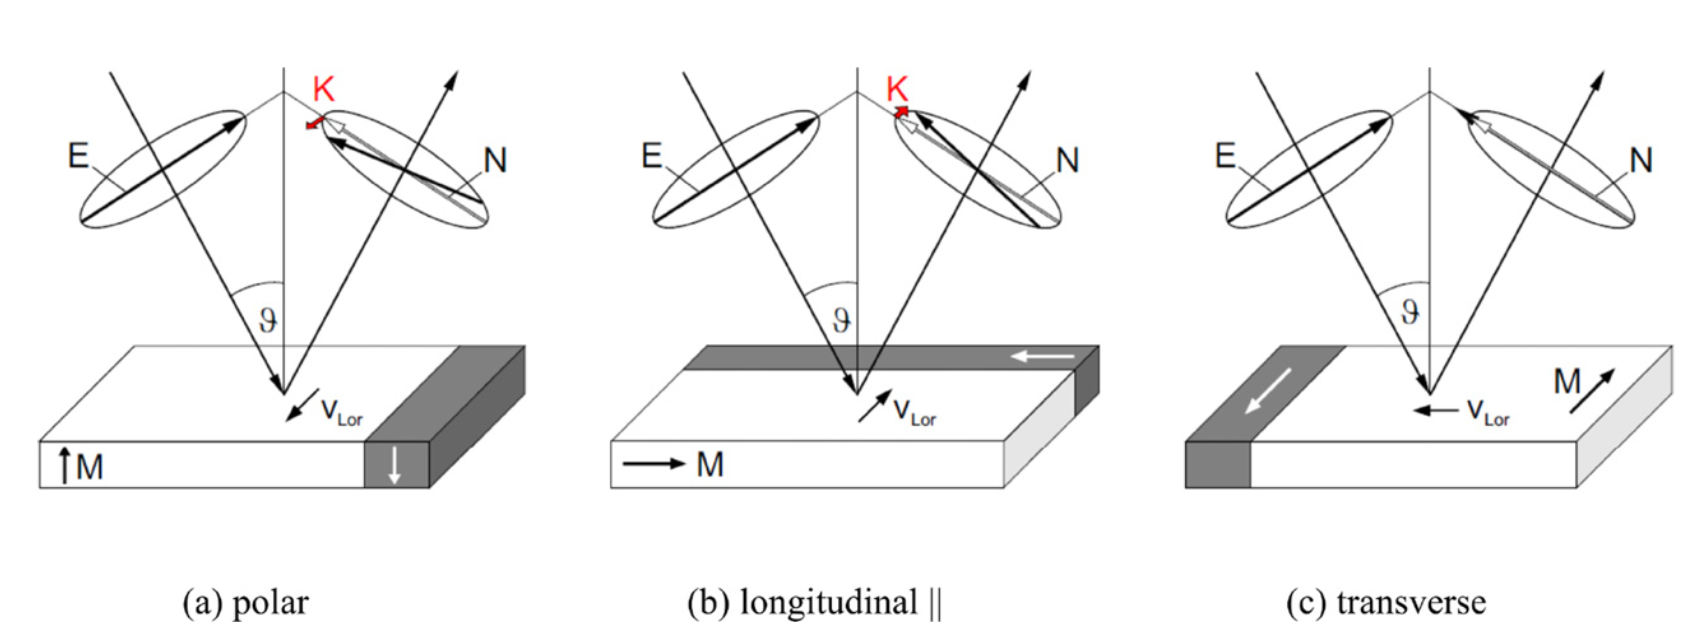
\includegraphics[width=0.8\textwidth]{fig1}
    \caption{Схематическое изображение конфигураций полярного, продольного и поперечного эффектов Керра, иллюстрирующих ориентацию вектора намагниченности $\mathbf{M}$ относительно падающего света.}
\end{figure}

\subsection{Ключевые принципы работы микроскопа Керра и количественный анализ}

МОЭК-микроскопия обычно использует поляризационный оптический микроскоп, где поляризатор создает линейно поляризованный падающий свет, а анализатор преобразует изменение поляризации отраженного света в контраст интенсивности.

\subsubsection{Интенсивность и создание контраста}
В широкопольной (wide-field) микроскопии Керра для создания контраста анализатор устанавливается в положение, близкое к скрещенному (почти гашение света).

Для количественной МОЭК-микроскопии отраженная интенсивность $I$ может быть аппроксимирована как линейная функция компонент намагниченности в плоскости образца:
$$
I = I_0 + Bm_l + Cm_t + D \quad \text{(1)}
$$
где:
\begin{itemize}
    \item $I_0$ — фоновая интенсивность, не зависящая от намагниченности.
    \item $m_l$ и $m_t$ — нормированные продольная и поперечная компоненты намагниченности (вдоль и перпендикулярно плоскости падения).
    \item $B$ и $C$ — коэффициенты, зависящие от нормальных ($N$) и керровских ($K$) амплитуд.
    \item $D$ — член второго порядка по намагниченности (квадратичный), порядка $K^2$.
\end{itemize}
В классическом подходе для наблюдения доменов, не зависящий от намагниченности вклад $I_0$ устраняется с помощью метода разностного изображения. При этом член $D$ (квадратичный по намагниченности) можно пренебречь, если анализатор и поляризатор настроены таким образом, что $N$ велик по сравнению с $K$.

\subsubsection{Векторная и количественная визуализация}
Для полного определения векторного поля намагниченности $\mathbf{M} = (m_x, m_y, m_z)$ в плоскости ($m_x, m_y$) необходимо получить два изображения с ортогональными чувствительностями. В современных микроскопах Керра это достигается путем:
\begin{enumerate}
    \item \textbf{Управления направлением падения:} Используется специальный источник света с массивом из восьми светодиодов, свет которых направляется через оптические волокна. Включение соответствующих светодиодов позволяет устанавливать направление падения света (и, следовательно, направление чувствительности Керра) без механических перемещений. Направление чувствительности (плоскость падения) определяется расположением источника света (концов волокон) в апертурной плоскости объектива.
    \item \textbf{Импульсный режим и вычитание:} Изображения записываются в импульсном режиме с поочередным включением противоположных светодиодов. Вычитание двух изображений, полученных при противоположных направлениях падения света, позволяет получить чистый плоскостной контраст Керра.
    \item \textbf{Устранение паразитного эффекта Фарадея:} Этот импульсный режим с вычитанием также эффективно устраняет паразитные вращения Фарадея, которые возникают в линзе объектива под действием внешнего магнитного поля и искажают сигнал МОЭК.
\end{enumerate}

\subsubsection{Процедура количественной реконструкции}
Количественный анализ требует регистрации двух синусоидальных калибровочных функций, сдвинутых по фазе на $90^\circ$, что обеспечивает два линейных уравнения для двух искомых компонент намагниченности $m_l$ и $m_t$.

В продвинутой методике, разработанной Soldatov и Schäfer, для устранения паразитных вкладов Фарадея и получения чистого контраста, используется разность интенсивностей $I_{\text{diff}}$:
$$
I_{\text{diff}} = I(H) - I(-H)
$$
где $I(H)$ и $I(-H)$ — интенсивности, измеренные при противоположных магнитных полях (или противоположных намагниченных состояниях).

Для реконструкции векторного поля намагниченности $\mathbf{M}$, количественная микроскопия Керра основывается на сравнении интенсивности каждого пикселя, измеренной при двух ортогональных чувствительностях, с локальными калибровочными функциями.

\begin{figure}[h]
    \centering
    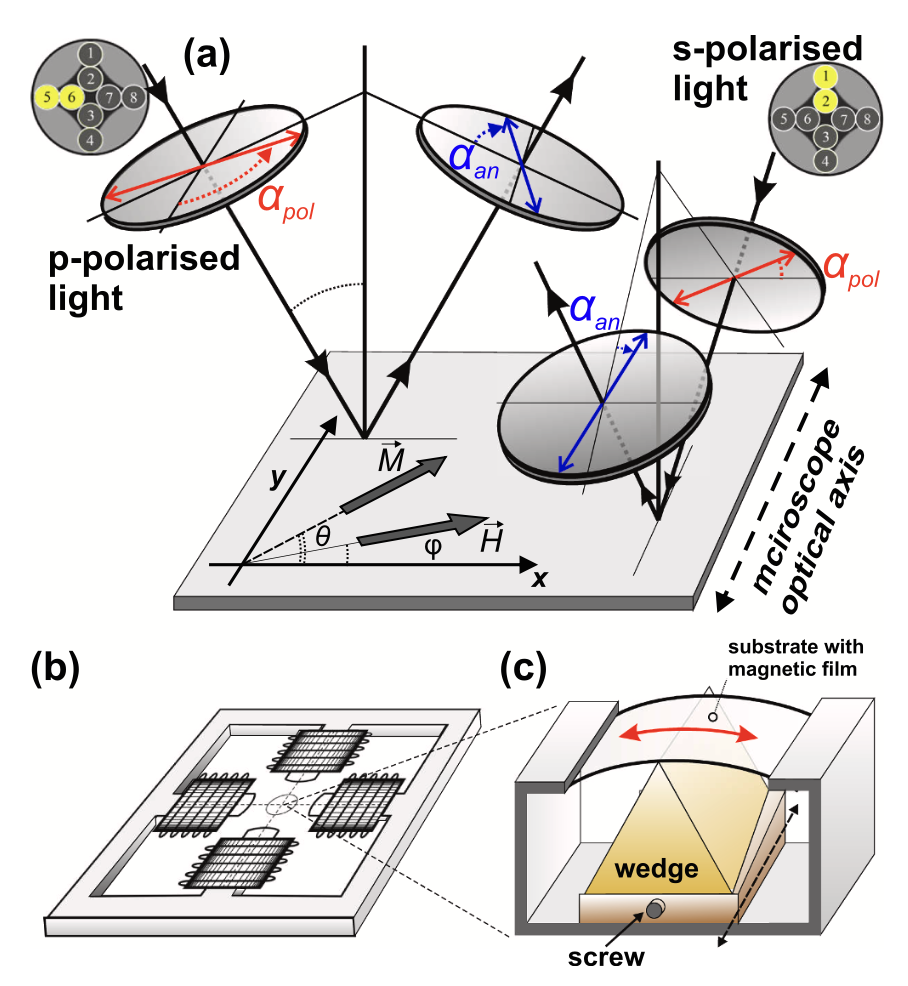
\includegraphics[width=0.8\textwidth]{fig2}
    \caption{Схематическое изображение установки широкопольного МОЭК-магнитометра, включающего массив светодиодов (LED cross), управляемых компьютером, для установки направления падения света и обеспечения ортогональных чувствительностей. (Источник: Рисунок 1(a) из "Advanced, Kerr-microscopy-based MOKE magnetometry for the anisotropy characterisation of magnetic films").}
\end{figure}

\section{Постановка задачи}

Физическая часть:
\begin{itemize}
  \item Аналитическое решение задачи.
  \item И тд.
\end{itemize}
Программная часть:
\begin{itemize}
  \item Реализация простого кроссплатформенного UI.
  \item Определения границ доменов с помощью машинного зрения. 
  \item Программное реализация. физических законов.
  \item И тд.
\end{itemize}

\section{Основная часть}

\subsection{Определения границ доменов}

Для анализа изображений магнитных доменов в образцах использовалась разработанная программная реализация метода, основанного на вычислении яркости пикселей и определении светлых и тёмных областей, соответствующих границам доменов.

Анализ начинается с получения матрицы яркости каждого пикселя изображения. Яркость вычисляется по формуле преобразования RGB-компонентов в яркостное значение:

\[
Y = 0.299 \cdot R + 0.587 \cdot G + 0.114 \cdot B
\]

Далее для каждого пикселя проводится классификация на основе пороговых значений яркости, выявляются светлые и тёмные границы доменов. Определяются ключевые точки границ и вычисляются центры доменов, а также векторные поля направлений на основе локальных свойств изображения.

Для визуализации результатов представлены две типовые микроскопические фотографии: исходная (\texttt{figdom1}) и та же фотография с нанесёнными границами доменов (\texttt{figdom2}).

\begin{figure}[H]
    \centering
    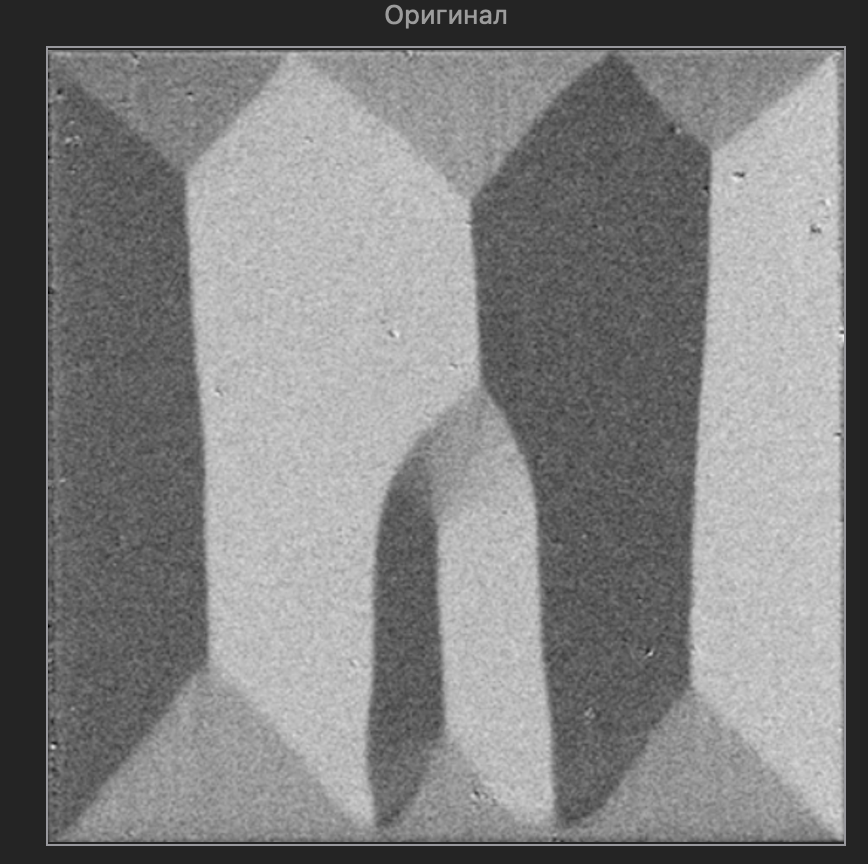
\includegraphics[width=0.8\linewidth]{figdom1}
    \caption{Исходное микроскопическое изображение магнитных доменов.}
    \label{fig:dom1}
\end{figure}

\begin{figure}[H]
    \centering
    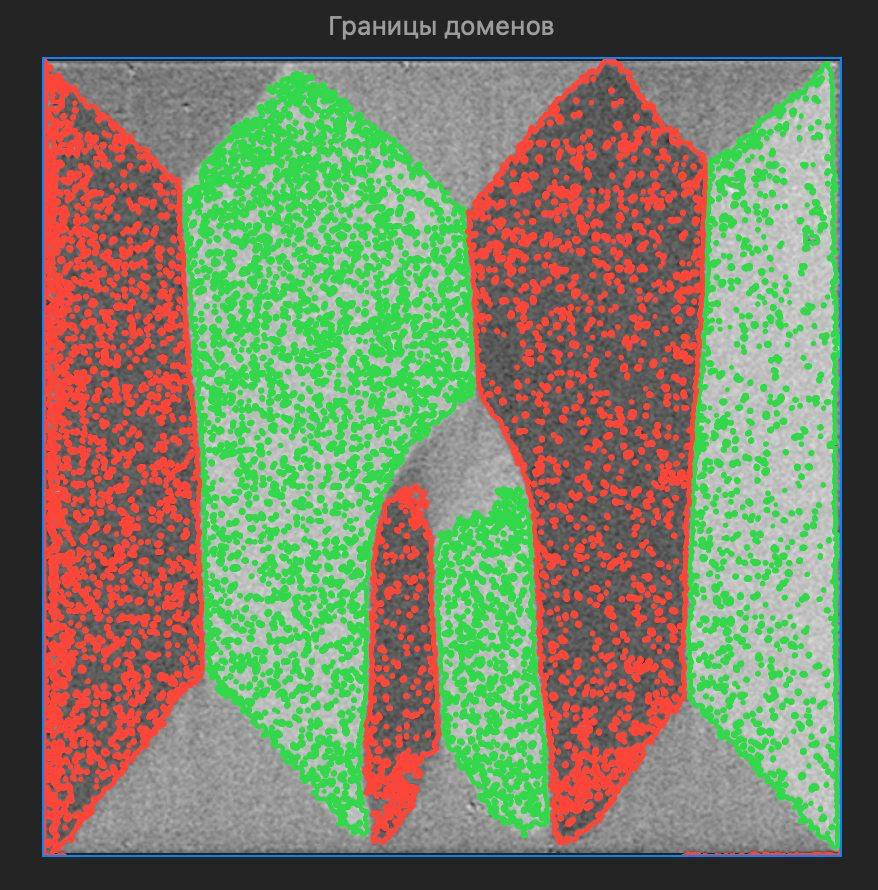
\includegraphics[width=0.8\linewidth]{figdom2}
    \caption{Микроскопическое изображение с наложенными границами доменов, выделенными программным методом.}
    \label{fig:dom2}
\end{figure}

\subsection*{Кратко о физической модели}
МОКЭ проявляется как вращение плоскости поляризации и эллиптичность отражённого света, линейно зависящие (в первом приближении) от соответствующей проекции \(\mathbf M\) на вектор чувствительности \(\mathbf b\), определяемый геометрией (полярной, продольной, поперечной) и оптической настройкой. В режиме «около экстинкции» сигнал фотоинтенсивности становится линейным по \(\rho_K\) и, следовательно, по компоненте \(\mathbf M\), на которую настроена система.

\subsection*{Нормировка и калибровка}
Применяется плоско-полевая коррекция \(I_0(x,y)\) и нормировка \(S=(I-I_0)/I_0\). Для установки абсолютного знака и масштаба выполняется дифференциальная съёмка на насыщении внешнего поля \(+H_{\text{sat}}\) и \(-H_{\text{sat}}\) с построением \(\Delta S\), что фиксирует \(\operatorname{sign}\) и оценивает \(\|\mathbf b\|\) при известной \(M_{\text{sat}}\). В области малого смещения анализатора на угол \(\delta\) от экстинкции интенсивность аппроксимируется
\[
 I_{\text{out}} \approx I_0\left(\delta^2 + 2\,\delta\,\operatorname{Re}\rho_K + |\rho_K|^2\right),
\]
и при \(|\rho_K|\ll \delta \ll 1\) линейная модель по \(\rho_K\) оправдана.

\subsection*{Один кадр и два кадра}
Для одного кадра определяется проекция \(M_{\text{sens}}=(S-a)/\|\mathbf b\|\) и маска доменов с учётом двузначности направления \(\pm\hat{\mathbf b}\). Для пары независимых кадров \(\mathbf b_1,\mathbf b_2\) решается система \(S-a=B\,\mathbf M\) с контролем обусловленности \(\kappa(B)\); при необходимости вводится регуляризация Тихонова.

\subsection*{Подавление шума и карта доверия}
Структурный тензор на изображении используется для оценки локальной когерентности и маскировки доменных стенок (как зон интенсивных градиентов), а также для задания весов уверенности. Визуализация включает векторное поле \(\mathbf M\) и карту доверия, легенду геометрии.

\subsection*{Валидация и метрики}
Используются: угловая ошибка \(\Delta\phi\) на тестовых объёмах и синтетике; метрики сегментации (IoU, F1); стабильность к дрейфу/шуму, проверка линейности при вариации \(\delta\); мониторинг \(\kappa(B)\) и размера регуляризации.

\section{Выводы}
\begin{itemize}
  \item Предложен воспроизводимый конвейер: нормировка → калибровка знака/масштаба → оценка проекции/вектора → маскирование стенок → визуализация и метрики.
  \item Реализуемость на Swift/Core Image/Accelerate подтверждена архитектурой модулей и набором метаданных для повторяемой съёмки и обработки.
  \item Введены критерии устойчивости и качества, позволяющие контролировать применимость линейной модели и корректность восстановления направления \(\mathbf M\).
\end{itemize}

\section*{Список литературы} \vspace{-4mm}
\begin{enumerate}
  \item Smith J. Example Article // Some Journal, 2022.
  \item Qiu Z. Q., Bader S. D. Surface magneto-optic Kerr effect // Journal of Magnetism and Magnetic Materials, 2000.
  \item Hubert A., Schäfer R. Magnetic Domains. Springer, 1998.
  \item Zvezdin A. K., Kotov V. A. Modern Magnetooptics and Magnetooptical Materials. Taylor \& Francis, 1997.
  \item Soldatov I. V., Schäfer R. Advanced MOKE magnetometry in wide-field Kerr-microscopy // J. Appl. Phys. 122, 153906 (2017).
  \item Soldatov I. V., Schäfer R. Selective sensitivity in Kerr microscopy // Rev. Sci. Instrum. 88, 073701 (2017).
  \item Soldatov I. V., Schäfer R. Advances in quantitative Kerr microscopy // Phys. Rev. B 95, 014426 (2017).
  \item Schäfer R. Investigation of domains and dynamics of domain walls by the magneto-optical Kerr-effect. In: Handbook of Magnetism and Advanced Magnetic Materials (John Wiley \& Sons, Ltd, 2007).
  \item Kuch W., Schäfer R., Fischer P., Hillebrecht F. Magnetic Microscopy of Layered Structures. Springer, New York, 2015.
  \item Schmidt F., Rave W., Hubert A. Enhancement of magneto-optical Domain observation by digital image-processing // IEEE Trans. Magn. 21, 1596 (1985).
  \item Faraday M. On the magnetisation of light and the illumination of magnetic lines of force // Philos. Trans. R. Soc. London 136, 1 (1846).
  \item Marko D., Soldatov I., Tekielak M., Schäfer R. Stray-field-induced Faraday contributions in wide-field Kerr microscopy and -magnetometry // J. Magn. Magn. Mater. 396, 9 (2015).
  \item Rave W., Reichel P., Brendel H., Leicht M., McCord J., Hubert A. Progress in quantitative magnetic domain observation // IEEE Trans. Magn. 29, 2551 (1993).
  \item Soldatov I., Zehner J., Leistner K., Kang T., Karnaushenko D., Schäfer R. Advanced, Kerr-microscopy-based MOKE magnetometry for the anisotropy characterisation of magnetic films // J. Magn. Magn. Mater. 529, 167889 (2021).
  \item Urs N. O., Mozooni B., Mazalski P., et al. Advanced magneto-optical microscopy: Imaging from picoseconds to centimeters - imaging spin waves and temperature distributions (invited) // AIP Advances 6, 055605 (2016).
  \item Schäfer R., Oppeneer P. M., Ognev A. V., et al. Analyzer-free, intensity-based, wide-field magneto-optical microscopy // Appl. Phys. Rev. 8, 031402 (2021).
  \item Oppeneer P. M. Magneto-optical Kerr spectra. In: Handbook of Magnetic Materials, Vol. 13 (Elsevier, 2001), pp. 229–422.
  \item Rave W., Schäfer R., Hubert A. Quantitative observation of magnetic domains with the magneto-optical Kerr effect // J. Magn. Magn. Mater. 65, 7 (1987).
  \item McCord J., Hubert A. Normalized differential Kerr microscopy an advanced method for magnetic imaging // Phys. Status Solidi A 171, 555–62 (1999).
  \item Wolf G., Hamrle J., Trudel S., et al. Quadratic magneto-optical Kerr effect in Co2MnSi // J. Appl. Phys. 110, 043904 (2011).
  \item Jiménez E., Mikuszeit N., Cuñado J. L. F., et al. Vectorial Kerr magnetometer for simultaneous and quantitative measurements of the in-plane magnetization components // Rev. Sci. Instrum. 85, 053904 (2014).
  \item Teixeira J. M., Lusche R., Ventura J., et al. Versatile, high sensitivity, and automatized angular dependent vectorial Kerr magnetometer for the analysis of nanostructured materials // Rev. Sci. Instrum. 82, 043902 (2011).
  \item Wu T.-h., Fu H., Hajjar R. A., Suzuki T., Mansuripur M. Measurement of magnetic anisotropy constant for magneto-optical recording media: A comparison of several techniques // J. Appl. Phys. 73, 1368–1376 (1993).
  \item Postava K., Jaffres H., Schuhl A., et al. Linear and quadratic magneto-optical measurements of the spin reorientation in epitaxial Fe films on MgO // J. Magn. Magn. Mater. 172, 199–208 (1997).
  \item Kerr J. On rotation of the plane of polarisation by reflection from the pole of a magnet // Philos. Mag. 3, 321–343 (1877).
\end{enumerate}

\newpage
\appendix

\section{Физическое приложение}
\subsection{Магнитооптический эффект Керра}
Магнитооптический эффект Керра — изменение поляризации отражённого света от намагниченного материала; наблюдаются вращение плоскости поляризации и эллиптичность, чувствительные к намагниченности в зоне зондирования света. В линейном по намагниченности приближении комплексный керровский угол \(\rho_K=\theta_K+i\epsilon_K\) при p-поляризованном падении аппроксимируется через элементы матрицы отражения как \(\rho_K\approx r_{ps}/r_{pp}\) (для s-падения \(\rho_K\approx r_{sp}/r_{ss}\)); чувствительность определяется внедиагональными компонентами диэлектрического тензора, пропорциональными компонентам \(\mathbf M\).

\subsection{Геометрии и чувствительность}
Рабочие геометрии МОКЭ и чувствительные компоненты \(\mathbf M\):
\begin{itemize}
  \item Полярная: чувствительна к внеплоскостной компоненте \(M_z\); удобна при близком к нормальному падении.
  \item Продольная: чувствительна к проекции в плоскости образца вдоль плоскости падения \(M_{\parallel}\).
  \item Поперечная: проявляется как изменение отражения \(\Delta R/R \propto M_{\perp}\) к плоскости падения; вращения плоскости поляризации нет.
\end{itemize}
При анализаторе около экстинкции фотосигнал становится к первой степени линейной функцией \(\rho_K\), что даёт линейную зависимость измеряемого сигнала от соответствующей проекции \(\mathbf M\).

\subsection{Магнитные домены и стенки}
Ферромагнитная плёнка разбивается на домены — области квази-единой ориентации \(\mathbf M\), разделённые доменными стенками с быстрым поворотом направления; МОКЭ-микроскопия визуализирует контраст доменов за счёт изменения \(\rho_K\) при смене компоненты \(\mathbf M\), на которую настроена чувствительность.

\subsection{Линейная модель сигнала и ограничения}
Введём нормированный сигнал \(S(x,y)\) после плоско-полевой калибровки:
\begin{equation}
 S(x,y)=\frac{I(x,y)-I_0(x,y)}{I_0(x,y)} \approx a + \mathbf b \cdot \mathbf M(x,y).
\end{equation}
Здесь \(\mathbf b\) — вектор чувствительности, задаваемый геометрией и настройкой поляризатор/анализатор. Одно изображение в фиксированной геометрии определяет лишь проекцию \(\mathbf M\) на \(\mathbf b\) и несёт двузначность \(\pm\) (на \(180^\circ\)) без дополнительной априорной информации (ориентации внешнего поля/калибровки).

\paragraph{Режим около экстинкции и линейность.}
Пусть анализатор смещён от экстинкции на малый угол \(\delta\). Тогда
\begin{equation}
 I_{\text{out}} \approx I_0\Big(\delta^2 + 2\,\delta\,\mathrm{Re}\,\rho_K + |\rho_K|^2\Big),
\end{equation}
и для \(|\rho_K| \ll \delta \ll 1\) вклад \(2\delta\,\mathrm{Re}\,\rho_K\) доминирует, обосновывая линейную аппроксимацию \(S\simeq a+\mathbf b\cdot\mathbf M\). Практически следует контролировать \(\delta\) в эксперименте и проверять линейность по серии малых \(\delta\).

\section{Математическое приложение}
\subsection{Постановка}
По входному МОКЭ-изображению \(I(x,y)\) и метаданным съёмки восстановить: при одном кадре — карту возможных направлений \(\pm\hat{\mathbf b}\) и знак проекции \(M_{\text{sens}}\); при двух независимых кадрах — вектор \((M_x,M_y)\) в плоскости образца.

\subsection{Нормировка и наблюдаемые}
Оценивается плоское поле \(I_0(x,y)\) и определяется
\begin{equation}
 S(x,y)=\frac{I(x,y)-I_0(x,y)}{I_0(x,y)}.
\end{equation}
Геометрия съёмки задаёт единичный \(\hat{\mathbf b}\) и масштаб \(\|\mathbf b\|\).

\subsection{Линейная модель и один кадр}
При фиксированной геометрии
\begin{equation}
 S(x,y)=a+\mathbf b\cdot \mathbf M(x,y).
\end{equation}
Оценка «чувствительной» проекции:
\begin{equation}
 M_{\text{sens}}(x,y)=\frac{S(x,y)-a}{\|\mathbf b\|}, \qquad \text{направление: } \pm \hat{\mathbf b}.
\end{equation}
Выводится карта знака и величины проекции с учётом двузначности.

\subsection{Два независимых кадра}
Для двух кадров с линейно независимыми \(\mathbf b_1,\mathbf b_2\) (в плоскости образца):
\begin{equation}
 \begin{bmatrix} S_1-a_1\\ S_2-a_2 \end{bmatrix}
 =
 \underbrace{\begin{bmatrix} b_{1x} & b_{1y}\\ b_{2x} & b_{2y}\end{bmatrix}}_{B}
 \begin{bmatrix} M_x\\ M_y \end{bmatrix}.
\end{equation}
Тогда \(\,(M_x,M_y)^\top = B^{-1}(S-a)\,\) при \(\det B\neq 0\). Для улучшения устойчивости при большой \(\kappa(B)\) используется
\begin{equation}
 \mathbf M = (B^\top B + \lambda I)^{-1}B^\top (S-a),
\end{equation}
где \(\lambda>0\) — малая регуляризация.

\subsection{Сегментация доменов}
Трёхзначная маска:
\begin{equation}
 D(x,y)=
 \begin{cases}
 +1, & M_{\text{sens}} > T,\\
 -1, & M_{\text{sens}} < -T,\\
 0, & |M_{\text{sens}}|\le T,
 \end{cases}
\end{equation}
где \(T\) — робастный порог (например, по MAD) после сглаживания и вычитания фона.

\subsection{Оценка локальной ориентации: структурный тензор}
Пусть \(I_x,I_y\) — градиенты. Структурный тензор
\begin{equation}
 J = G_\rho * 
 \begin{bmatrix}
 I_x^2 & I_x I_y\\
 I_x I_y & I_y^2
 \end{bmatrix}.
\end{equation}
Угол локальной ориентации
\begin{equation}
 \phi = \tfrac12 \arctan2\!\big(2J_{xy},\, J_{xx}-J_{yy}\big),
\end{equation}
когерентность 
\begin{equation}
 c=\frac{\lambda_1-\lambda_2}{\lambda_1+\lambda_2},
\end{equation}
где \(\lambda_1\ge\lambda_2\) — собственные значения \(J\). Значение \(c\) используется для подавления шумовых областей и маскировки доменных стенок.

\subsection{Предобработка и устойчивость}
Применяются: гауссово сглаживание \(G_\sigma * I\), вычитание медленного фона, морфологические операции (open/close), адаптивный порог; доверие пикселя по \(|S|\) и \(c\). Эти шаги стабилизируют знак и границы доменов перед визуализацией.

\subsection{Калибровка на насыщении и знак}
Снимается пара кадров при \(+H_{\text{sat}}\) и \(-H_{\text{sat}}\) в неизменной геометрии:
\begin{equation}
 \Delta S = S(+H_{\text{sat}})-S(-H_{\text{sat}}) \approx 2\,\|\mathbf b\|\,M_{\text{sat}}\cdot \operatorname{sign}.
\end{equation}
Это задаёт абсолютный знак и позволяет оценить \(\|\mathbf b\|\) при известном \(M_{\text{sat}}\). Рекомендуется сохранять \(\Delta S\) как эталон для серии.

\subsection{Проверка независимости и ковариация}
Линейная независимость \(\mathbf b_1,\mathbf b_2\) контролируется по \(|\det B|\) и \(\kappa(B)\). При гауссовском шуме с ковариацией \(\Sigma\) ковариация оценки
\begin{equation}
 \mathrm{Cov}(\mathbf M) \approx (B^\top \Sigma^{-1} B)^{-1}.
\end{equation}
Это используется для построения карты доверия и отбора пикселей.

\subsection{Псевдокод конвейера}
\begin{enumerate}
  \item Стабилизация и flat-field: оценить \(I_0\), получить \(S=(I-I_0)/I_0\).
  \item Калибровка: снять \(\Delta S\) на \(\pm H_{\text{sat}}\), установить знак и \(\|\mathbf b\|\).
  \item Один кадр: \(M_{\text{sens}}=(S-a)/\|\mathbf b\|\), пороговая маска после сглаживания.
  \item Два кадра: собрать \(S_1,S_2\), проверить \(\kappa(B)\), восстановить \(\mathbf M\) с регуляризацией при необходимости.
  \item Структурный тензор: посчитать \(c\), замаскировать стенки и шумовые зоны.
  \item Визуализация: карта знака/вектора, карта доверия, легенда геометрии.
\end{enumerate}

\section{Программное приложение}

Для практической реализации алгоритмов анализа магнитных доменов было разработано приложение для операционной системы macOS. Приложение написано на языке Swift с использованием фреймворка SwiftUI для построения пользовательского интерфейса.

\subsection{Архитектура приложения}

Проект построен по модульному принципу, разделяя логику обработки данных и пользовательский интерфейс. Структура проекта включает три основных компонента:
\begin{itemize}
    \item \textbf{course4\_programApp.swift} --- точка входа в приложение.
    \item \textbf{ContentView.swift} --- описание пользовательского интерфейса и взаимодействия с пользователем.
    \item \textbf{generateVectorDiagram.swift} --- реализация алгоритмов обработки изображений и анализа доменов.
\end{itemize}

Полный листинг исходного кода приведен в разделе \ref{sec:code_listing}.

\subsection{Алгоритмы обработки и анализа}

Ядром приложения является модуль \texttt{generateVectorDiagram.swift} (см. Листинг \ref{lst:logic}). Процесс обработки изображения состоит из нескольких этапов.

\subsubsection{Предобработка и кэширование}
При загрузке изображения оно преобразуется в матрицу яркости (Grayscale). Поскольку операции вычисления порогов и фильтрации могут требовать ресурсов, реализован механизм кэширования через класс \texttt{ImageAnalysisCache} (Листинг~\ref{lst:logic}, \hyperref[logic:cache]{строки 11--34}). Функция \texttt{createAnalysisCache} (\hyperref[logic:createcache]{строки 152--222}) выполняет первичную обработку, в ходе которой вычисляются и сохраняются:
\begin{itemize}
    \item Матрица яркости пикселей (\hyperref[logic:matrix]{строки 175--191}).
    \item Минимальное и максимальное значения яркости (\hyperref[logic:minmax]{строки 180--190}).
    \item Базовые пороги сегментации, вычисленные автоматически (\hyperref[logic:basethresh]{строки 208--221}).
\end{itemize}
Яркость пикселя вычисляется по стандартной формуле преобразования RGB в Grayscale (\hyperref[logic:brightness]{строки 163--173}):
\[
Y = 0.299 \cdot R + 0.587 \cdot G + 0.114 \cdot B
\]
Это позволяет быстрее пересчитывать результаты при ручной корректировке параметров пользователем без повторного чтения данных изображения.

\subsubsection{Автоматическая пороговая сегментация (Метод Оцу)}
Для автоматического определения границ доменов реализован модифицированный двухуровневый метод Оцу (функция \texttt{otsuDualThreshold}, Листинг~\ref{lst:logic}, \hyperref[logic:otsu]{строки 43--149}). Алгоритм находит два оптимальных порога, разделяющих пиксели на три класса:
\begin{enumerate}
    \item Тёмные области (домены одного направления).
    \item Светлые области (домены противоположного направления).
    \item Нейтральные области (переходные зоны, границы, шум).
\end{enumerate}
Для повышения устойчивости к шуму перед вычислением гистограммы отбрасываются по 5\% самых темных и самых светлых пикселей (trimming, \hyperref[logic:trim]{строки 62--91}). Оптимизация порогов выполняется путём максимизации межклассовой дисперсии (\hyperref[logic:variance]{строки 115--142}).

\subsubsection{Сегментация и фильтрация доменов}
Функция \texttt{analyzeDomains} (Листинг~\ref{lst:logic}, \hyperref[logic:analyze]{строки 225--406}) выполняет сегментацию изображения на основе порогов. Пользователь имеет возможность корректировать пороги относительно базовых значений Оцу с помощью коэффициентов (от $0.8$ до $1.2$), что реализовано через функцию \texttt{applySliderMultiplier} (\hyperref[logic:slider]{строки 37--40}). Применение порогов выполняется в \hyperref[logic:applythresh]{строках 234--235}.

Для выделения связных областей используется алгоритм поиска в ширину (BFS, \hyperref[logic:bfs]{строки 257--304}). Пиксели группируются в домены, после чего применяется фильтрация по размеру: области, занимающие менее $1/5000$ площади изображения, считаются шумом и отбрасываются (\hyperref[logic:filter]{строки 307--308}).

\subsubsection{Построение векторной диаграммы}
Для каждого выделенного домена вычисляется его центроид (\hyperref[logic:centroid]{строки 370--381}). В зависимости от классификации домена (светлый или темный) ему приписывается условное направление вектора намагниченности (в текущей реализации — вверх или вниз, отображаемые красным и синим цветами соответственно, \hyperref[logic:direction]{строки 386--398}). Также алгоритм определяет пиксели границ доменов для их визуализации: граничными считаются пиксели, имеющие соседей из другого домена или находящиеся на краю изображения (\hyperref[logic:boundary]{строки 333--366}).

\subsection{Пользовательский интерфейс}

Интерфейс приложения (файл \texttt{ContentView.swift}, Листинг~\ref{lst:ui}) предоставляет следующие возможности:
\begin{itemize}
    \item Загрузка изображений форматов PNG и JPEG (функция \texttt{openImageFile}, \hyperref[ui:openfile]{строки 233--246}).
    \item Визуализация исходного изображения (\hyperref[ui:original]{строки 110--120}).
    \item Панель настроек с ползунками для точной подстройки порогов сегментации <<на лету>> (\hyperref[ui:sliders]{строки 68--103}).
    \item Режим наложения результатов анализа: отображение границ доменов (\hyperref[ui:boundaries]{строки 123--141}) и векторного поля (\hyperref[ui:vectorfield]{строки 143--156}) поверх оригинального изображения.
\end{itemize}
Для эффективной отрисовки большого количества графических примитивов используются специализированные компоненты на базе \texttt{Canvas}: \texttt{ArrowFieldView} для отрисовки стрелок (\hyperref[ui:arrowfield]{строки 181--193}) и \texttt{DomainBoundaryView} для отрисовки точек границ (\hyperref[ui:domainboundary]{строки 196--225}), обеспечивающие высокую производительность.

\newpage
\section{Листинг программного кода} \label{sec:code_listing}

\subsection{Точка входа (course4\_programApp.swift)}
\begin{lstlisting}[language=Swift, caption=Точка входа в приложение, label=lst:main]
//
//  course4_programApp.swift
//  course4_program
//

import SwiftUI

@main
struct course4_programApp: App {
    var body: some Scene {
        WindowGroup {
            ContentView()
        }
    }
}
\end{lstlisting}

\subsection{Интерфейс пользователя (ContentView.swift)}
\begin{lstlisting}[language=Swift, caption=Пользовательский интерфейс, label=lst:ui]
import SwiftUI
import UniformTypeIdentifiers
import AppKit

struct ContentView: View {
    @State private var image: NSImage?
    @State private var vectorArrows: [Arrow] = []

    @State private var brightBoundaryPoints: [CGPoint] = []
    @State private var darkBoundaryPoints: [CGPoint] = []

    @State private var showVectorDiagram: Bool = false

    // Кэш анализа изображения (яркость + базовые пороги Otsu)
    @State private var analysisCache: ImageAnalysisCache?

    // Ползунки: 0..1, где 0.5 = значение Otsu
    // При 0: порог×0.8, при 1: порог×1.2
    @State private var darkSlider: Double = 0.5
    @State private var brightSlider: Double = 0.5

    private let canvasSize: CGFloat = 400

    var body: some View {
        VStack(spacing: 16) {

            HStack(spacing: 12) {
                Button("Загрузить изображение") {
                    openImageFile { selectedImage in
                        self.image = selectedImage
                        self.vectorArrows = []
                        self.brightBoundaryPoints = []
                        self.darkBoundaryPoints = []
                        self.showVectorDiagram = false
                        self.analysisCache = nil
                        // Сброс ползунков на середину
                        self.darkSlider = 0.5
                        self.brightSlider = 0.5
                    }
                }

                Button("Векторная диаграмма") {
                    guard let img = image else { return }
                    
                    // Создаём кэш, если его ещё нет
                    if analysisCache == nil {
                        analysisCache = createAnalysisCache(from: img)
                    }
                    
                    guard let cache = analysisCache else { return }
                    
                    let vis = analyzeDomains(
                        cache: cache,
                        targetSize: canvasSize,
                        darkSlider: darkSlider,
                        brightSlider: brightSlider
                    )
                    self.vectorArrows = vis.arrows
                    self.brightBoundaryPoints = vis.brightBoundaryPoints
                    self.darkBoundaryPoints = vis.darkBoundaryPoints
                    self.showVectorDiagram = true
                }
                .disabled(image == nil)
            }
            .padding(.top, 16)

            // Ползунки для настройки порогов (*@\label{ui:sliders}@*)
            // 0 = base×0.8, 0.5 = base (Otsu), 1 = base×1.2
            VStack(spacing: 8) {
                HStack {
                    Text("Порог тёмных:")
                        .frame(width: 120, alignment: .leading)
                    Text("×0.80")
                        .font(.caption)
                        .foregroundColor(.secondary)
                    Slider(value: $darkSlider, in: 0...1)
                        .frame(width: 180)
                    Text("×1.20")
                        .font(.caption)
                        .foregroundColor(.secondary)
                    Text(sliderMultiplierText(darkSlider))
                        .frame(width: 50, alignment: .trailing)
                        .font(.caption)
                }

                HStack {
                    Text("Порог ярких:")
                        .frame(width: 120, alignment: .leading)
                    Text("×0.80")
                        .font(.caption)
                        .foregroundColor(.secondary)
                    Slider(value: $brightSlider, in: 0...1)
                        .frame(width: 180)
                    Text("×1.20")
                        .font(.caption)
                        .foregroundColor(.secondary)
                    Text(sliderMultiplierText(brightSlider))
                        .frame(width: 50, alignment: .trailing)
                        .font(.caption)
                }
            }
            .padding(.horizontal)

            Divider()

            ScrollView {
                if let nsImage = image {
                    VStack(spacing: 24) {

                        VStack(spacing: 8) { (*@\label{ui:original}@*)
                            Text("Оригинал")
                                .foregroundColor(.secondary)

                            Image(nsImage: nsImage)
                                .resizable()
                                .scaledToFit()
                                .frame(width: canvasSize, height: canvasSize)
                                .border(Color.gray)
                        }

                        if showVectorDiagram {

                            VStack(spacing: 8) { (*@\label{ui:boundaries}@*)
                                Text("Границы доменов")
                                    .foregroundColor(.secondary)

                                Image(nsImage: nsImage)
                                    .resizable()
                                    .scaledToFit()
                                    .frame(width: canvasSize, height: canvasSize)
                                    .overlay(
                                        DomainBoundaryView(
                                            brightPoints: brightBoundaryPoints,
                                            darkPoints: darkBoundaryPoints
                                        )
                                        .frame(width: canvasSize, height: canvasSize)
                                        .allowsHitTesting(false)
                                    )
                                    .border(Color.blue)
                            }

                            VStack(spacing: 8) { (*@\label{ui:vectorfield}@*)
                                Text("Векторное поле")
                                    .foregroundColor(.secondary)

                                Image(nsImage: nsImage)
                                    .resizable()
                                    .scaledToFit()
                                    .frame(width: canvasSize, height: canvasSize)
                                    .overlay(
                                        ArrowFieldView(arrows: vectorArrows)
                                            .frame(width: canvasSize, height: canvasSize)
                                            .allowsHitTesting(false)
                                    )
                                    .border(Color.blue)
                            }
                        }
                    }
                    .frame(maxWidth: .infinity)
                    .padding(.bottom, 24)
                } else {
                    Text("Файл не выбран")
                        .foregroundColor(.secondary)
                        .frame(maxWidth: .infinity, maxHeight: .infinity)
                        .padding()
                }
            }
        }
        .frame(minWidth: 600, minHeight: 800)
        .padding()
    }
}

struct Arrow {
    var start: CGPoint
    var end: CGPoint
    var color: Color
}

struct ArrowFieldView: View { (*@\label{ui:arrowfield}@*)
    var arrows: [Arrow]

    var body: some View {
        Canvas { context, size in
            for arrow in arrows {
                var path = Path()
                path.move(to: arrow.start)
                path.addLine(to: arrow.end)
                context.stroke(path, with: .color(arrow.color), lineWidth: 2)
            }
        }
    }
}

struct DomainBoundaryView: View { (*@\label{ui:domainboundary}@*)
    var brightPoints: [CGPoint] // зелёные
    var darkPoints: [CGPoint]   // красные

    var body: some View {
        Canvas { context, size in
            let dotSize: CGFloat = 2.0

            for p in brightPoints {
                let rect = CGRect(
                    x: p.x - dotSize / 2,
                    y: p.y - dotSize / 2,
                    width: dotSize,
                    height: dotSize
                )
                context.fill(Path(ellipseIn: rect), with: .color(.green))
            }

            for p in darkPoints {
                let rect = CGRect(
                    x: p.x - dotSize / 2,
                    y: p.y - dotSize / 2,
                    width: dotSize,
                    height: dotSize
                )
                context.fill(Path(ellipseIn: rect), with: .color(.red))
            }
        }
    }
}

/// Форматирование множителя для отображения
func sliderMultiplierText(_ slider: Double) -> String {
    let multiplier = 0.8 + slider * 0.4
    return String(format: "%.2f", multiplier)
}

func openImageFile(completion: @escaping (NSImage?) -> Void) { (*@\label{ui:openfile}@*)
    let panel = NSOpenPanel()
    panel.allowedContentTypes = [.png, .jpeg]
    panel.allowsMultipleSelection = false
    panel.canChooseDirectories = false

    if panel.runModal() == .OK,
       let url = panel.url,
       let nsImage = NSImage(contentsOf: url) {
        completion(nsImage)
    } else {
        completion(nil)
    }
}
\end{lstlisting}

\subsection{Логика анализа (generateVectorDiagram.swift)}
\begin{lstlisting}[language=Swift, caption=Алгоритмы обработки, label=lst:logic]
import SwiftUI
import AppKit

struct DomainVisualization {
    let arrows: [Arrow]
    let brightBoundaryPoints: [CGPoint]  // границы светлых доменов
    let darkBoundaryPoints: [CGPoint]    // границы тёмных доменов
}

/// Кэш для хранения данных анализа изображения (*@\label{logic:cache}@*)
class ImageAnalysisCache {
    let brightness: [[Double]]
    let width: Int
    let height: Int
    let minB: Double
    let maxB: Double
    let range: Double
    
    // Базовые пороги, рассчитанные методом Otsu (абсолютные значения яркости)
    let baseDarkThreshold: Double
    let baseBrightThreshold: Double
    
    init(brightness: [[Double]], width: Int, height: Int, minB: Double, maxB: Double,
         baseDarkThreshold: Double, baseBrightThreshold: Double) {
        self.brightness = brightness
        self.width = width
        self.height = height
        self.minB = minB
        self.maxB = maxB
        self.range = maxB - minB
        self.baseDarkThreshold = baseDarkThreshold
        self.baseBrightThreshold = baseBrightThreshold
    }
}

/// Применение линейного множителя к порогу (*@\label{logic:slider}@*)
func applySliderMultiplier(baseValue: Double, slider: Double) -> Double {
    let multiplier = 0.8 + slider * 0.4
    return baseValue * multiplier
}

/// Двухпороговый метод Otsu для разделения на 3 класса (*@\label{logic:otsu}@*)
func otsuDualThreshold(brightness: [[Double]], width: Int, height: Int, trimPercent: Double = 0.05) -> (dark: Double, bright: Double) {
    let numBins = 256
    var histogram = [Int](repeating: 0, count: numBins)
    var totalPixels = 0

    // Построение полной гистограммы
    for y in 0..<height {
        for x in 0..<width {
            let br = brightness[y][x]
            let bin = min(numBins - 1, max(0, Int(br * Double(numBins - 1))))
            histogram[bin] += 1
            totalPixels += 1
        }
    }

    guard totalPixels > 0 else {
        return (dark: 0.33, bright: 0.66)
    }

    // Вычисление перцентилей для отбрасывания крайних значений (*@\label{logic:trim}@*)
    let trimCount = Int(Double(totalPixels) * trimPercent)
    var lowBin = 0
    var highBin = numBins - 1
    
    var cumSum = 0
    for i in 0..<numBins {
        cumSum += histogram[i]
        if cumSum >= trimCount {
            lowBin = i
            break
        }
    }
    
    cumSum = 0
    for i in stride(from: numBins - 1, through: 0, by: -1) {
        cumSum += histogram[i]
        if cumSum >= trimCount {
            highBin = i
            break
        }
    }
    
    var trimmedHistogram = [Int](repeating: 0, count: numBins)
    var trimmedTotalPixels = 0
    
    for i in lowBin...highBin {
        trimmedHistogram[i] = histogram[i]
        trimmedTotalPixels += histogram[i]
    }
    
    guard trimmedTotalPixels > 0 else {
        return (dark: 0.33, bright: 0.66)
    }

    var prob = [Double](repeating: 0, count: numBins)
    var cumProb = [Double](repeating: 0, count: numBins)
    var cumMean = [Double](repeating: 0, count: numBins)

    for i in 0..<numBins {
        prob[i] = Double(trimmedHistogram[i]) / Double(trimmedTotalPixels)
    }

    cumProb[0] = prob[0]
    cumMean[0] = 0

    for i in 1..<numBins {
        cumProb[i] = cumProb[i - 1] + prob[i]
        cumMean[i] = cumMean[i - 1] + Double(i) * prob[i]
    }

    let totalMean = cumMean[numBins - 1]

    var maxVariance = -1.0 (*@\label{logic:variance}@*)
    var bestT1 = numBins / 3
    var bestT2 = 2 * numBins / 3

    let step = max(1, numBins / 64)
    
    for t1 in stride(from: 1, to: numBins - 2, by: step) {
        for t2 in stride(from: t1 + 1, to: numBins - 1, by: step) {
            let w0 = cumProb[t1]
            let w1 = cumProb[t2] - cumProb[t1]
            let w2 = 1.0 - cumProb[t2]

            if w0 <= 0 || w1 <= 0 || w2 <= 0 { continue }

            let mu0 = cumMean[t1] / w0
            let mu1 = (cumMean[t2] - cumMean[t1]) / w1
            let mu2 = (totalMean - cumMean[t2]) / w2

            let variance = w0 * (mu0 - totalMean) * (mu0 - totalMean) +
                          w1 * (mu1 - totalMean) * (mu1 - totalMean) +
                          w2 * (mu2 - totalMean) * (mu2 - totalMean)

            if variance > maxVariance {
                maxVariance = variance
                bestT1 = t1
                bestT2 = t2
            }
        }
    }

    let darkThreshold = Double(bestT1) / Double(numBins - 1)
    let brightThreshold = Double(bestT2) / Double(numBins - 1)

    return (dark: darkThreshold, bright: brightThreshold)
}

/// Создание кэша анализа изображения (*@\label{logic:createcache}@*)
func createAnalysisCache(from image: NSImage) -> ImageAnalysisCache? {
    guard
        let tiffData = image.tiffRepresentation,
        let bitmap = NSBitmapImageRep(data: tiffData)
    else {
        return nil
    }

    let width = bitmap.pixelsWide
    let height = bitmap.pixelsHigh

    func brightnessAt(x: Int, y: Int) -> Double? { (*@\label{logic:brightness}@*)
        guard
            let color = bitmap.colorAt(x: x, y: y)?
                .usingColorSpace(NSColorSpace.deviceRGB)
        else { return nil }

        let r = Double(color.redComponent)
        let g = Double(color.greenComponent)
        let b = Double(color.blueComponent)
        return 0.299 * r + 0.587 * g + 0.114 * b
    }

    var brightness: [[Double]] = Array( (*@\label{logic:matrix}@*)
        repeating: Array(repeating: 0.0, count: width),
        count: height
    )

    var minB = 1.0 (*@\label{logic:minmax}@*)
    var maxB = 0.0

    for y in 0..<height {
        for x in 0..<width {
            if let br = brightnessAt(x: x, y: y) {
                brightness[y][x] = br
                if br < minB { minB = br }
                if br > maxB { maxB = br }
            }
        }
    }

    guard maxB > minB else {
        return nil
    }

    let range = maxB - minB
    var normalizedBrightness: [[Double]] = Array(
        repeating: Array(repeating: 0.0, count: width),
        count: height
    )
    for y in 0..<height {
        for x in 0..<width {
            normalizedBrightness[y][x] = (brightness[y][x] - minB) / range
        }
    }

    let thresholds = otsuDualThreshold(brightness: normalizedBrightness, width: width, height: height) (*@\label{logic:basethresh}@*)
    
    let baseDarkThreshold = minB + thresholds.dark * range
    let baseBrightThreshold = minB + thresholds.bright * range

    return ImageAnalysisCache(
        brightness: brightness,
        width: width,
        height: height,
        minB: minB,
        maxB: maxB,
        baseDarkThreshold: baseDarkThreshold,
        baseBrightThreshold: baseBrightThreshold
    )
}

/// Анализ доменов (*@\label{logic:analyze}@*)
func analyzeDomains(cache: ImageAnalysisCache,
                    targetSize: CGFloat = 400,
                    darkSlider: Double = 0.5,
                    brightSlider: Double = 0.5) -> DomainVisualization {

    let width = cache.width
    let height = cache.height
    let brightness = cache.brightness

    let tDark = applySliderMultiplier(baseValue: cache.baseDarkThreshold, slider: darkSlider) (*@\label{logic:applythresh}@*)
    let tBright = applySliderMultiplier(baseValue: cache.baseBrightThreshold, slider: brightSlider)

    struct Domain {
        var points: [(Int, Int)]
        var isBright: Bool
        var index: Int
    }

    var labels = Array(
        repeating: Array(repeating: -1, count: width),
        count: height
    )

    var domains: [Domain] = []

    let neighbors = [
        (dx: 1,  dy: 0),
        (dx: -1, dy: 0),
        (dx: 0,  dy: 1),
        (dx: 0,  dy: -1)
    ]

    for y in 0..<height { (*@\label{logic:bfs}@*)
        for x in 0..<width {
            let br = brightness[y][x]
            let isBright = br >= tBright
            let isDark = br <= tDark

            if !(isBright || isDark) { continue }
            if labels[y][x] != -1 { continue }

            let classIsBright = isBright
            let labelIndex = domains.count

            var queue: [(Int, Int)] = []
            var pts: [(Int, Int)] = []

            labels[y][x] = labelIndex
            queue.append((x, y))

            while !queue.isEmpty {
                let (cx, cy) = queue.removeFirst()
                pts.append((cx, cy))

                for n in neighbors {
                    let nx = cx + n.dx
                    let ny = cy + n.dy

                    if nx < 0 || nx >= width || ny < 0 || ny >= height { continue }
                    if labels[ny][nx] != -1 { continue }

                    let nbr = brightness[ny][nx]
                    let nIsBright = nbr >= tBright
                    let nIsDark = nbr <= tDark

                    if classIsBright {
                        if !nIsBright { continue }
                    } else {
                        if !nIsDark { continue }
                    }

                    labels[ny][nx] = labelIndex
                    queue.append((nx, ny))
                }
            }

            domains.append(
                Domain(points: pts, isBright: classIsBright, index: labelIndex)
            )
        }
    }

    let minDomainPixels = max(50, (width * height) / 5000) (*@\label{logic:filter}@*)
    let filteredDomains = domains.filter { $0.points.count >= minDomainPixels }

    let imageAspect = CGFloat(width) / CGFloat(height)
    var displayWidth: CGFloat
    var displayHeight: CGFloat
    var offsetX: CGFloat = 0
    var offsetY: CGFloat = 0

    if imageAspect > 1.0 {
        displayWidth = targetSize
        displayHeight = targetSize / imageAspect
        offsetY = (targetSize - displayHeight) / 2
    } else {
        displayHeight = targetSize
        displayWidth = targetSize * imageAspect
        offsetX = (targetSize - displayWidth) / 2
    }

    let scaleX = displayWidth / CGFloat(width)
    let scaleY = displayHeight / CGFloat(height)

    var arrows: [Arrow] = []
    var brightBoundaryPoints: [CGPoint] = []
    var darkBoundaryPoints: [CGPoint] = []

    for domain in filteredDomains { (*@\label{logic:boundary}@*)
        let labelIndex = domain.index

        for (x, y) in domain.points {
            var isBoundary = false

            for n in neighbors {
                let nx = x + n.dx
                let ny = y + n.dy

                if nx < 0 || nx >= width || ny < 0 || ny >= height {
                    isBoundary = true
                    break
                }

                if labels[ny][nx] != labelIndex {
                    isBoundary = true
                    break
                }
            }

            if isBoundary {
                let px = CGFloat(x) * scaleX + offsetX
                let py = CGFloat(y) * scaleY + offsetY
                let p = CGPoint(x: px, y: py)

                if domain.isBright {
                    brightBoundaryPoints.append(p)
                } else {
                    darkBoundaryPoints.append(p)
                }
            }
        }
    }

    let baseLength: CGFloat = 40

    for domain in filteredDomains { (*@\label{logic:centroid}@*)
        var sumX = 0.0
        var sumY = 0.0

        for (x, y) in domain.points {
            sumX += Double(x)
            sumY += Double(y)
        }

        let count = Double(domain.points.count)
        let cx = sumX / count
        let cy = sumY / count

        let sx = CGFloat(cx) * scaleX + offsetX
        let sy = CGFloat(cy) * scaleY + offsetY

        let dir: CGFloat = domain.isBright ? 1.0 : -1.0 (*@\label{logic:direction}@*)
        let ex = sx
        let ey = sy + dir * baseLength

        let color: Color = domain.isBright ? .red : .blue

        arrows.append(
            Arrow(
                start: CGPoint(x: sx, y: sy),
                end: CGPoint(x: ex, y: ey),
                color: color
            )
        )
    }

    return DomainVisualization(
        arrows: arrows,
        brightBoundaryPoints: brightBoundaryPoints,
        darkBoundaryPoints: darkBoundaryPoints
    )
}
\end{lstlisting}

\end{document}


